\chapter{조사 지역 및 언어}

\section{지역의 특징}

조사 장소인 벌교읍은 전라남도 보성군의 최동단에 위치한 행정구역이다. 면적은 102.58 km²이며, 71개의 행정리와 166개의 반으로 구성되어 있다. 2022년 기준 내외국인 6,416가구, 11,474명이 거주하고 있다.

\begin{figure}[h]
    \centering
    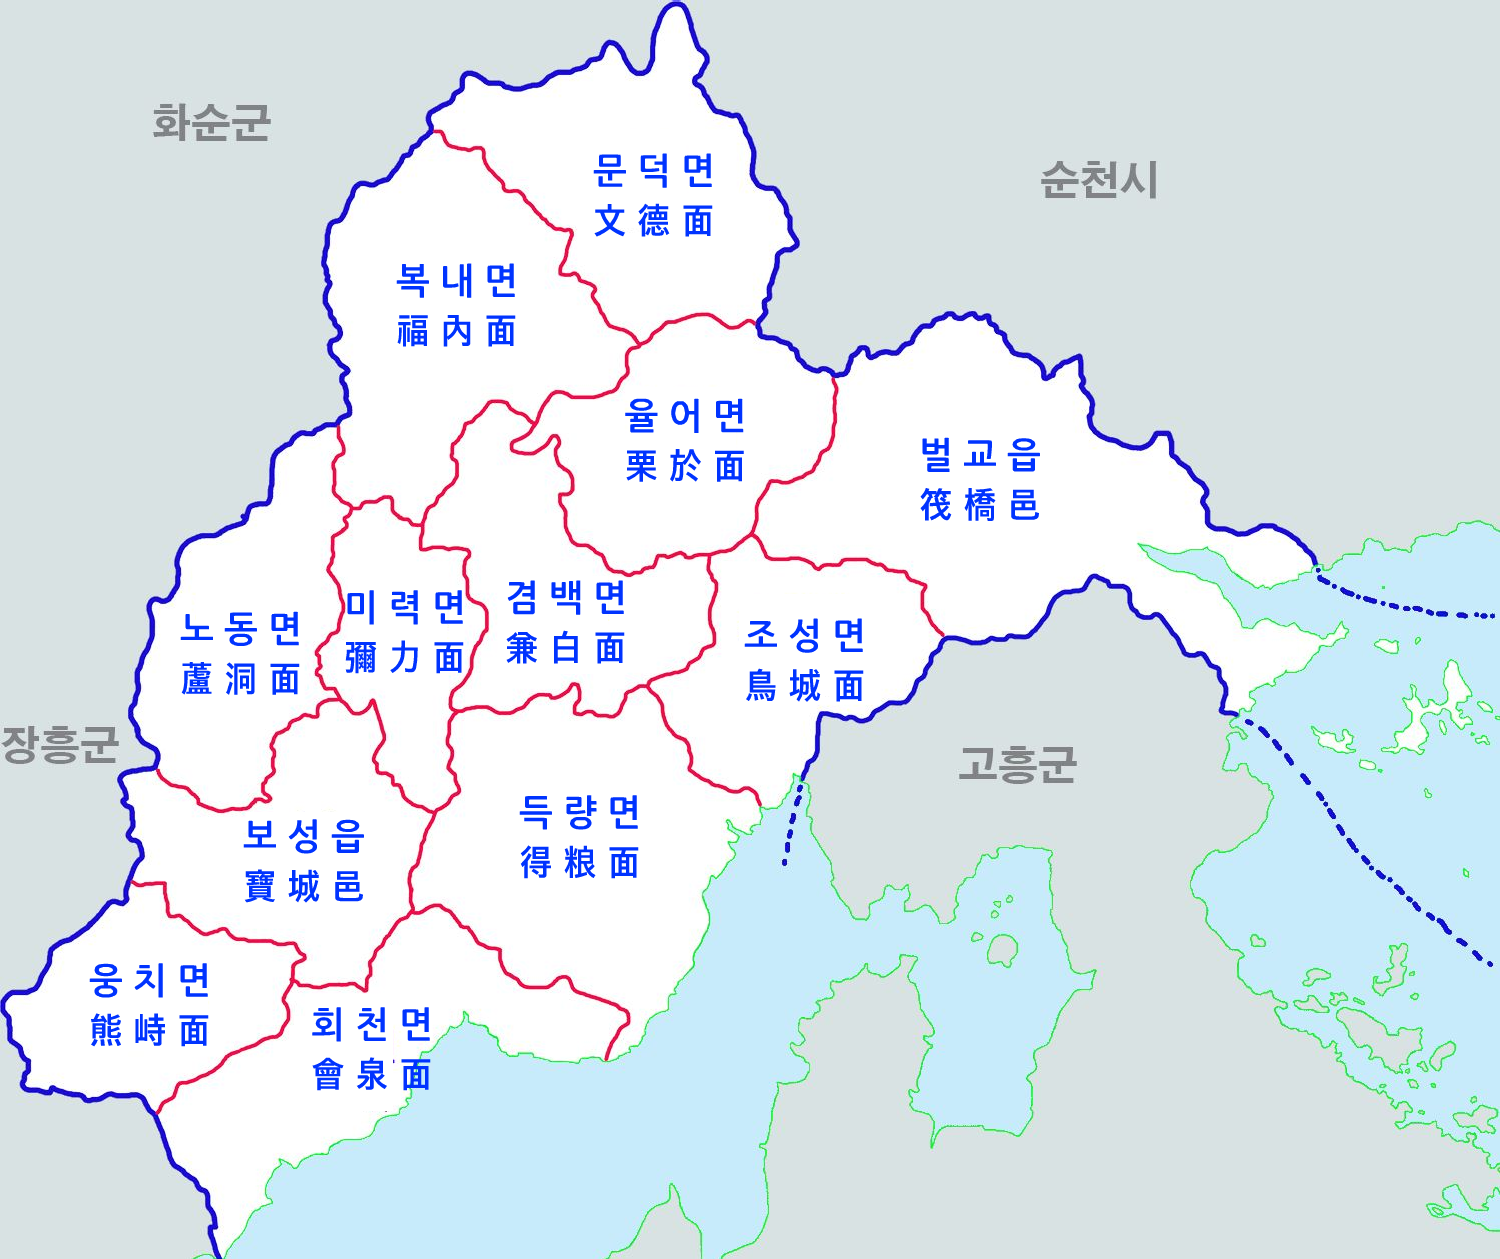
\includegraphics[width=0.5\textwidth]{images/boseong-map.png}
\end{figure}

본래 벌교 일대는 순천 낙안읍성으로도 잘 알려진 낙안군에 속해 있었다. 그러나 1908년, 일제에 의해 혼란해진 국세 속에서 낙안군이 폐지되면서 그 남단의 고상면, 고하면, 남상면, 남하면 4개 면이 보성군으로 통합되었는데, 이후 순천군 동하면(전 낙안군 동하면)까지 통합되면서 이루어진 것이 벌교면, 곧 현재의 벌교읍이다.

이러한 배경 속에서 벌교읍은 비록 행정적으로 보성군에 속할지언정, 어떤 면에서는 인접한 순천시 일대와 더 가까운 독자적인 문화 및 생활권을 유지하고 있다. 자연지리적으로 보아도 벌교읍은 인근의 순천시 낙안면과 함께 침식분지인 낙안분지에 속하여 있는데, 이는 전체적으로 산맥의 비중이 높은 보성군에서 이질적인 특징이다.

벌교읍은 조선 시대부터 이어져 온 어업 중심지인 한편, 일제강점기 개항으로 상업에 있어서도 비교적 번화하게 되었다. 순천만 연안 전반의 특산물이던 꼬막은 현재 `벌교 꼬막'으로서 지역적 아이덴티티를 대표하고 있으며, 이외에 조정래의 단편소설 《태백산맥》, 2003년 영화 《황산벌》 등 대중 매체에서도 벌교의 특색을 어렵잖게 살필 수 있다.

\section{언어의 특징}

보성군에 속해 있으나 많은 측면에서 인접한 순천시에 더 가깝다는 벌교의 역사문화적 특징은 그 언어를 파악하는 데 있어 큰 난관으로 다가온다. 서남 방언의 하위 구획에서, 보성 방언과 순천 방언은 차이가 매우 큰 것으로 보고되기 때문이다.\footnote{정성훈. (2017). 서남방언의 하위방언구획과 네트워크 분석. 언어학, 77, 157-180.}

전남 방언은 크게 동부와 서부, 또 북부와 남부로 나눌 수 있다. 이때 벌교 방언은 보성읍 전반, 순천시 서부와 같은 남부 방언권, 동시에 순천시와는 같지만 보성읍 전반과는 다른 동부 방언권으로 분류된다. 따라서 사전 조사 과정에서 조사자들은 전남 동남부 방언, 특히 순천 방언에 대한 선행 연구를 중심으로 벌교의 언어적 특징을 파악하고자 하였다.

전통적인 전남 동부 방언은 `ㅣ, ㅔ, ㅐ, ㅟ, ㅚ, ㅡ, ㅓ, ㅏ, ㅜ, ㅗ'의 10모음 체계를 가진 것으로 간주되며,\footnote{이기갑. (1986). 전라남도의 언어지리. 서울: 탑출판사.} 특히 `떼'와 `때', `(가방을) 메다'와 `(끈을) 매다', `(풀을) 베다'와 `(아이를) 배다' 등 최소대립쌍이 존재하는 것으로 보고되어 있다.\footnote{방언연구회. (2001). 방언학 사전. 서울: 태학사.} 반면 전남 서부 방언은 `ㅔ'가 `ㅐ'와 합류한 9모음 체계를 가진 것으로 보고된다. 동부 방언과 서부 방언을 통틀어, 어간 내부뿐만 아니라 용언의 피·사동형 및 활용형, 체언의 곡용형에서도 움라우트로 인한 모음 상승 현상이 관찰된다.\footnote{이돈주. (1987). 전남 방언의 특징과 그 연구. 국어생활, 8, 64-79.}

역사적 자음 약화의 양상도 동부와 서부 방언에서 다른 것으로 확인되는데,\footnote{이기갑(1986).} `ㄹ' 뒤 `ㄱ'가 유성음화되어 탈락한 변화, `ㅂ'가 일부 환경에서 순경음을 거쳐 탈락한 변화는 서부에서만 일어난 것으로 보인다. 이에 따르면 벌교 방언에서는 중세 국어의 소리 있는 `ㅇ'이 `ㄱ'으로, `ㅸ'이 `ㅂ'으로 대응될 것이 기대되는데, 특히 `부추'를 가리키는 `솔/소불' 등 특징적 어휘의 출현 여부에 주목할 수 있다.

전남 일부 지역에서는 `부풀다'에 대한 `부크다', `주걱'에 대한 `주벅', `차곡차곡'에 대한 `차복차복' 등 소위 PK교체 현상이 확인된다. 다만 역시 지역에 따라 보고되는 어형의 차이가 커 벌교 방언의 양상을 특정하기에는 어렵다.

중세어에서 비자동적 어간 교체를 보이던 일부 어휘(`구무\textasciitilde{}구ᇚ[穴]' 등)는 두 이형태가 의미상 분화하여 다른 지시물을 가리키게 된 정황이 포착된다.\footnote{이돈주(1987).} 나아가, `ㄷ' 불규칙 용언이 `고' 앞에서 `ㄹ'을 가지고 쓰이는 `물꼬/물코(묻고)'와 같은 형태도 보고되어 있다.\footnote{이진숙. (2019).  전라남도 방언구획을 위한 방언분화 연구(1) -음운론적 측면을 중심으로-. 방언학, 30, 169-198.} 불규칙 곡용·활용 패러다임에 대한 검토가 필요할 것이다.

마지막으로, 전통적 서남 방언에는 특징적 경어 체계가 존재한다. 상대 높임의 선어말어미 `-이-'와 `-습-'이 보고되며,\footnote{이기갑. (1991). 표준어와 서남 방언. 새국어생활, 1(3), 73-82.} 종결어미 체계는 `허씨요체-허소체-해라체'의 삼분이 가능하다. 세 말씨는 모두 [-격식성]을 띄는바 중앙어의 체계와 곧바로 대응되지 않는다.\footnote{박양규. (1980). 서남방언 경어법의 한 문제: 이른바 주체존대법에 나타나는 `-게'의 경우. 방언, 3, 27-45.} 전남 서부에서는 아주높임의 `-게라', `-라우', 높임의 `-게'가 보고되는데,\footnote{이진숙(2019).} 벌교 방언에서 이들 어미가 확인될지 여부는 명확하지 않다.

벌교의 언어가 이질적 특징을 가질 것으로 기대되는 데에 반해, 그를 특정하여 이루어진 선행 연구는 많지 않다. 본 조사가 서남 방언의 채록이라는 일차적 목적을 넘어서, 벌교의 고유한 언어적 특징을 파악할 단초를 제공해 주지는 않을까 희망하여 본다.
